\documentclass[11pt]{article}
\usepackage[margin=1in]{geometry}
\usepackage[T1]{fontenc}
\usepackage{textcomp}
\usepackage{amsmath,amssymb,booktabs,graphicx,setspace,caption,threeparttable}
\usepackage[round,authoryear]{natbib}
\usepackage[hidelinks]{hyperref}
\captionsetup{font=small,labelfont=bf}
\onehalfspacing
\newcommand{\fignote}[1]{\par\vspace{2pt}{\footnotesize\emph{Notes:} #1\par}}
% generated by code/31_numbers.py - do not edit
\newcommand{\ageOldB}{104.3}
\newcommand{\ageOldP}{0.029}
\newcommand{\ageOldSE}{46.9}
\newcommand{\auditCorrect}{95}
\newcommand{\auditN}{100}
\newcommand{\caCc}{0.97}
\newcommand{\caGt}{1.18}
\newcommand{\caRe}{1.58}
\newcommand{\caSt}{0.72}
\newcommand{\corrGasForced}{-0.02}
\newcommand{\corrGasFuel}{-0.39}
\newcommand{\corrGasFuelLev}{-0.64}
\newcommand{\corrGasOther}{-0.01}
\newcommand{\corrGasPlanned}{-0.06}
\newcommand{\coxGTHR}{0.98}
\newcommand{\coxGTP}{0.931}
\newcommand{\coxN}{773}
\newcommand{\coxOldHR}{0.72}
\newcommand{\coxOldP}{0.024}
\newcommand{\coxPrivHR}{1.22}
\newcommand{\coxPrivN}{69}
\newcommand{\coxPrivP}{0.081}
\newcommand{\coxSteamHR}{0.72}
\newcommand{\coxSteamP}{0.063}
\newcommand{\coxUnspecHR}{0.89}
\newcommand{\coxUnspecP}{0.305}
\newcommand{\demB}{-0.60}
\newcommand{\demSE}{0.26}
\newcommand{\dhakaBias}{1.4}
\newcommand{\dhakaR}{0.81}
\newcommand{\eforAllCc}{0.130}
\newcommand{\eforAllGt}{0.343}
\newcommand{\eforAllSt}{0.075}
\newcommand{\eforNoneCc}{0.073}
\newcommand{\eforNoneGt}{0.230}
\newcommand{\eforNoneSt}{0.048}
\newcommand{\eforShedCc}{0.154}
\newcommand{\eforShedGt}{0.409}
\newcommand{\eforShedSt}{0.136}
\newcommand{\eforTenCc}{0.130}
\newcommand{\eforTenGt}{0.342}
\newcommand{\eforTenSt}{0.074}
\newcommand{\fuelCoal}{1.000}
\newcommand{\fuelDays}{650}
\newcommand{\fuelGas}{0.994}
\newcommand{\fuelOil}{0.992}
\newcommand{\gtTopThreeShare}{75}
\newcommand{\heatOnsetCcgtIRR}{0.92}
\newcommand{\heatOnsetCcgtIRRHi}{1.13}
\newcommand{\heatOnsetCcgtIRRLo}{0.75}
\newcommand{\heatOnsetCcgtIRRP}{0.445}
\newcommand{\heatOnsetIRR}{0.86}
\newcommand{\heatOnsetIRRHi}{0.95}
\newcommand{\heatOnsetIRRLo}{0.78}
\newcommand{\heatOnsetIRRP}{0.004}
\newcommand{\heatOnsets}{304}
\newcommand{\heatOnsetsHot}{23}
\newcommand{\heatTripCcgtIRR}{1.04}
\newcommand{\heatTripCcgtIRRHi}{1.09}
\newcommand{\heatTripCcgtIRRLo}{0.99}
\newcommand{\heatTripCcgtIRRP}{0.150}
\newcommand{\heatTripIRR}{1.04}
\newcommand{\heatTripIRRHi}{1.08}
\newcommand{\heatTripIRRLo}{0.99}
\newcommand{\heatTripIRRP}{0.116}
\newcommand{\heatTrips}{828}
\newcommand{\heatTripsHot}{66}
\newcommand{\heatUnitDays}{66,821}
\newcommand{\hotTripCcgtIRR}{1.44}
\newcommand{\hotTripCcgtIRRHi}{2.45}
\newcommand{\hotTripCcgtIRRLo}{0.84}
\newcommand{\hotTripCcgtIRRP}{0.183}
\newcommand{\hotTripIRR}{1.50}
\newcommand{\hotTripIRRHi}{2.39}
\newcommand{\hotTripIRRLo}{0.94}
\newcommand{\hotTripIRRP}{0.088}
\newcommand{\ieeeCcEAF}{0.80}
\newcommand{\ieeeCcEAFomc}{0.71}
\newcommand{\ieeeCcEFOR}{0.130}
\newcommand{\ieeeCcFOR}{0.073}
\newcommand{\ieeeCcInactive}{4}
\newcommand{\ieeeCcMTBF}{290}
\newcommand{\ieeeCcMTTRmean}{29}
\newcommand{\ieeeCcMTTRmed}{3}
\newcommand{\ieeeCcPrivEAF}{0.91}
\newcommand{\ieeeCcPrivEFOR}{0.012}
\newcommand{\ieeeCcPrivMTBF}{1,272}
\newcommand{\ieeeCcPubEAF}{0.78}
\newcommand{\ieeeCcPubEFOR}{0.161}
\newcommand{\ieeeCcPubMTBF}{238}
\newcommand{\ieeeGtEAF}{0.74}
\newcommand{\ieeeGtEAFomc}{0.62}
\newcommand{\ieeeGtEFOR}{0.343}
\newcommand{\ieeeGtFOR}{0.230}
\newcommand{\ieeeGtInactive}{8}
\newcommand{\ieeeGtMTBF}{105}
\newcommand{\ieeeGtMTTRmean}{50}
\newcommand{\ieeeGtMTTRmed}{1}
\newcommand{\ieeeReEAF}{0.93}
\newcommand{\ieeeReEAFomc}{0.88}
\newcommand{\ieeeReEFOR}{0.081}
\newcommand{\ieeeReFOR}{0.010}
\newcommand{\ieeeReInactive}{0}
\newcommand{\ieeeReMTBF}{657}
\newcommand{\ieeeReMTTRmean}{7}
\newcommand{\ieeeReMTTRmed}{1}
\newcommand{\ieeeStEAF}{0.81}
\newcommand{\ieeeStEAFomc}{0.58}
\newcommand{\ieeeStEFOR}{0.075}
\newcommand{\ieeeStFOR}{0.048}
\newcommand{\ieeeStInactive}{27}
\newcommand{\ieeeStMTBF}{347}
\newcommand{\ieeeStMTTRmean}{18}
\newcommand{\ieeeStMTTRmed}{6}
\newcommand{\inactNinetyCcEAF}{0.83}
\newcommand{\inactNinetyCcShare}{9}
\newcommand{\inactNinetyGtEAF}{0.75}
\newcommand{\inactNinetyGtShare}{14}
\newcommand{\inactNinetyStEAF}{0.86}
\newcommand{\inactNinetyStShare}{34}
\newcommand{\inactNoneCcEAF}{0.80}
\newcommand{\inactNoneCcShare}{0}
\newcommand{\inactNoneGtEAF}{0.75}
\newcommand{\inactNoneGtShare}{0}
\newcommand{\inactNoneStEAF}{0.71}
\newcommand{\inactNoneStShare}{0}
\newcommand{\inactOneEightyCcEAF}{0.83}
\newcommand{\inactOneEightyCcShare}{4}
\newcommand{\inactOneEightyGtEAF}{0.75}
\newcommand{\inactOneEightyGtShare}{8}
\newcommand{\inactOneEightyStEAF}{0.83}
\newcommand{\inactOneEightyStShare}{27}
\newcommand{\inactThreeSixFiveCcEAF}{0.81}
\newcommand{\inactThreeSixFiveCcShare}{2}
\newcommand{\inactThreeSixFiveGtEAF}{0.74}
\newcommand{\inactThreeSixFiveGtShare}{3}
\newcommand{\inactThreeSixFiveStEAF}{0.81}
\newcommand{\inactThreeSixFiveStShare}{23}
\newcommand{\lapCcDet}{5}
\newcommand{\lapCcImp}{5}
\newcommand{\lapCcTested}{31}
\newcommand{\lapGtDet}{4}
\newcommand{\lapGtImp}{1}
\newcommand{\lapGtTested}{16}
\newcommand{\lapReDet}{8}
\newcommand{\lapReImp}{1}
\newcommand{\lapReTested}{22}
\newcommand{\lapStDet}{1}
\newcommand{\lapStImp}{5}
\newcommand{\lapStTested}{9}
\newcommand{\nCheckDays}{2,575}
\newcommand{\nDays}{2,577}
\newcommand{\nPrivCcgt}{9}
\newcommand{\nRemarks}{1,058}
\newcommand{\nTrips}{1,587}
\newcommand{\nTripsLinked}{1,442}
\newcommand{\nTripsStated}{775}
\newcommand{\nUndated}{30}
\newcommand{\nUnitDays}{409,029}
\newcommand{\nUnits}{225}
\newcommand{\newUnitB}{5.2}
\newcommand{\newUnitP}{0.258}
\newcommand{\newUnitSE}{4.6}
\newcommand{\onsetRateNineteen}{1.7}
\newcommand{\onsetRateTwenty}{2.3}
\newcommand{\onsetRateTwentyFour}{5.3}
\newcommand{\ownCcgtB}{-58.9}
\newcommand{\ownCcgtMean}{55.6}
\newcommand{\ownCcgtN}{40,025}
\newcommand{\ownCcgtP}{0.064}
\newcommand{\ownCcgtPrivUnits}{8}
\newcommand{\ownCcgtPw}{0.082}
\newcommand{\ownCcgtSE}{30.8}
\newcommand{\ownCcgtTripB}{-4.7}
\newcommand{\ownCcgtTripMean}{17.7}
\newcommand{\ownCcgtTripN}{37,283}
\newcommand{\ownCcgtTripP}{0.217}
\newcommand{\ownCcgtTripPrivUnits}{8}
\newcommand{\ownCcgtTripPw}{0.360}
\newcommand{\ownCcgtTripSE}{3.7}
\newcommand{\ownCcgtTripUnits}{34}
\newcommand{\ownCcgtUnits}{34}
\newcommand{\ownForcedB}{-81.1}
\newcommand{\ownForcedMean}{89.4}
\newcommand{\ownForcedN}{67,786}
\newcommand{\ownForcedP}{0.025}
\newcommand{\ownForcedPrivUnits}{10}
\newcommand{\ownForcedPw}{0.020}
\newcommand{\ownForcedSE}{35.4}
\newcommand{\ownForcedUnits}{70}
\newcommand{\ownFuelIdleB}{-1.4}
\newcommand{\ownFuelIdleMean}{11.8}
\newcommand{\ownFuelIdleN}{106,343}
\newcommand{\ownFuelIdleP}{0.776}
\newcommand{\ownFuelIdlePrivUnits}{10}
\newcommand{\ownFuelIdleSE}{4.9}
\newcommand{\ownFuelIdleUnits}{79}
\newcommand{\ownLooHi}{-66.7}
\newcommand{\ownLooLo}{-93.8}
\newcommand{\ownNoSteamB}{-82.2}
\newcommand{\ownNoSteamMean}{96.1}
\newcommand{\ownNoSteamN}{58,311}
\newcommand{\ownNoSteamP}{0.049}
\newcommand{\ownNoSteamPrivUnits}{8}
\newcommand{\ownNoSteamPw}{0.031}
\newcommand{\ownNoSteamSE}{40.9}
\newcommand{\ownNoSteamUnits}{53}
\newcommand{\ownNonfuelB}{-6.8}
\newcommand{\ownNonfuelMean}{14.5}
\newcommand{\ownNonfuelN}{93,094}
\newcommand{\ownNonfuelP}{0.054}
\newcommand{\ownNonfuelPrivUnits}{10}
\newcommand{\ownNonfuelPw}{0.072}
\newcommand{\ownNonfuelSE}{3.5}
\newcommand{\ownNonfuelUnits}{71}
\newcommand{\ownTripB}{-5.6}
\newcommand{\ownTripMean}{12.8}
\newcommand{\ownTripN}{60,864}
\newcommand{\ownTripP}{0.087}
\newcommand{\ownTripPrivUnits}{10}
\newcommand{\ownTripPw}{0.146}
\newcommand{\ownTripSE}{3.2}
\newcommand{\ownTripUnits}{68}
\newcommand{\ownZeroB}{-13.0}
\newcommand{\ownZeroExclB}{-8.3}
\newcommand{\ownZeroExclMean}{32.0}
\newcommand{\ownZeroExclN}{99,570}
\newcommand{\ownZeroExclP}{0.128}
\newcommand{\ownZeroExclPrivUnits}{10}
\newcommand{\ownZeroExclPw}{0.158}
\newcommand{\ownZeroExclSE}{5.4}
\newcommand{\ownZeroExclUnits}{79}
\newcommand{\ownZeroMean}{42.4}
\newcommand{\ownZeroN}{117,663}
\newcommand{\ownZeroP}{0.034}
\newcommand{\ownZeroPrivUnits}{10}
\newcommand{\ownZeroPw}{0.056}
\newcommand{\ownZeroSE}{6.0}
\newcommand{\ownZeroUnits}{79}
\newcommand{\rainCtrl}{1.01}
\newcommand{\rainCtrlHi}{1.22}
\newcommand{\rainCtrlLo}{0.84}
\newcommand{\rainCtrlN}{41}
\newcommand{\rainCtrlP}{0.925}
\newcommand{\rainElec}{1.15}
\newcommand{\rainElecHi}{1.24}
\newcommand{\rainElecLo}{1.07}
\newcommand{\rainElecN}{90}
\newcommand{\rainElecP}{<0.001}
\newcommand{\rainFuel}{1.09}
\newcommand{\rainFuelHi}{1.20}
\newcommand{\rainFuelLo}{0.99}
\newcommand{\rainFuelN}{162}
\newcommand{\rainFuelP}{0.092}
\newcommand{\rainGrid}{1.06}
\newcommand{\rainGridHi}{1.22}
\newcommand{\rainGridLo}{0.93}
\newcommand{\rainGridN}{31}
\newcommand{\rainGridP}{0.371}
\newcommand{\rainLpmB}{0.09}
\newcommand{\rainLpmSE}{0.03}
\newcommand{\rainMech}{1.02}
\newcommand{\rainMechHi}{1.13}
\newcommand{\rainMechLo}{0.92}
\newcommand{\rainMechN}{101}
\newcommand{\rainMechP}{0.756}
\newcommand{\rainOnsetIRR}{1.00}
\newcommand{\rainOnsetIRRHi}{1.10}
\newcommand{\rainOnsetIRRLo}{0.91}
\newcommand{\rainOnsetIRRP}{0.956}
\newcommand{\rainTripCcgtIRR}{1.05}
\newcommand{\rainTripCcgtIRRHi}{1.09}
\newcommand{\rainTripCcgtIRRLo}{1.01}
\newcommand{\rainTripCcgtIRRP}{0.011}
\newcommand{\rainTripIRR}{1.07}
\newcommand{\rainTripIRRHi}{1.10}
\newcommand{\rainTripIRRLo}{1.03}
\newcommand{\rainTripIRRP}{<0.001}
\newcommand{\resHighShed}{40}
\newcommand{\resLowShed}{198}
\newcommand{\resNoShed}{2,079}
\newcommand{\spForced}{526}
\newcommand{\spForcedMedian}{2}
\newcommand{\spInactive}{31}
\newcommand{\spMaintunspecified}{453}
\newcommand{\spPlanned}{12}
\newcommand{\spPlannedMedian}{27}
\newcommand{\spUnspecMedian}{4}
\newcommand{\tmaxSDraw}{4.2}
\newcommand{\tmaxSDwithin}{1.6}
\newcommand{\tripBoiler}{67}
\newcommand{\tripControl}{54}
\newcommand{\tripCooling}{25}
\newcommand{\tripElectrical}{132}
\newcommand{\tripFuelsupply}{202}
\newcommand{\tripGrid}{66}
\newcommand{\tripMean}{12.4}
\newcommand{\tripOther}{154}
\newcommand{\tripRateNineteen}{16.1}
\newcommand{\tripRateTwentyFour}{8.6}
\newcommand{\tripTurbine}{75}
\newcommand{\tripUnstated}{812}
\newcommand{\warmOnsetIRR}{0.73}
\newcommand{\warmOnsetIRRHi}{1.09}
\newcommand{\warmOnsetIRRLo}{0.48}
\newcommand{\warmOnsetIRRP}{0.124}
\newcommand{\warmOnsetPholm}{0.372}
\newcommand{\wbBootCcHi}{0.82}
\newcommand{\wbBootCcLo}{0.73}
\newcommand{\wbBootGtHi}{0.82}
\newcommand{\wbBootGtLo}{0.60}
\newcommand{\wbBootReHi}{0.69}
\newcommand{\wbBootReLo}{0.51}
\newcommand{\wbBootStHi}{0.95}
\newcommand{\wbBootStLo}{0.71}
\newcommand{\wbCc}{0.76}
\newcommand{\wbCcEta}{35}
\newcommand{\wbCcHi}{0.81}
\newcommand{\wbCcLo}{0.72}
\newcommand{\wbGt}{0.69}
\newcommand{\wbGtEta}{48}
\newcommand{\wbGtHi}{0.77}
\newcommand{\wbGtLo}{0.64}
\newcommand{\wbRe}{0.57}
\newcommand{\wbReEta}{86}
\newcommand{\wbReHi}{0.63}
\newcommand{\wbReLo}{0.53}
\newcommand{\wbSt}{0.78}
\newcommand{\wbStEta}{46}
\newcommand{\wbStHi}{0.91}
\newcommand{\wbStLo}{0.70}
\newcommand{\wbUnitCc}{0.90}
\newcommand{\wbUnitCcLt}{77}
\newcommand{\wbUnitCcN}{30}
\newcommand{\wbUnitGt}{0.99}
\newcommand{\wbUnitGtLt}{55}
\newcommand{\wbUnitGtN}{11}
\newcommand{\wbUnitRe}{0.49}
\newcommand{\wbUnitReLt}{100}
\newcommand{\wbUnitReN}{7}
\newcommand{\wbUnitSt}{0.89}
\newcommand{\wbUnitStLt}{75}
\newcommand{\wbUnitStN}{4}


\title{\textbf{Operational Reliability of a Gas-Constrained Thermal Fleet:\\ Evidence from Unit-Level Dispatch Reports in Bangladesh}}
\author{Tanvir Thamid\thanks{Independent researcher. E-mail: tanvirthamid@gmail.com. All data are public: the daily reports of the National Load Dispatch Centre published by the Bangladesh Power Development Board, NASA POWER weather data, BPDB annual reports and the WRI Global Power Plant Database. The code that collects, parses and analyses them, and that generates every number in the text, is archived with the paper. \emph{Declaration of generative AI use:} a generative AI system (Claude, Anthropic) was used extensively in this work, to write and run the code for data collection, parsing and statistical analysis and to draft and edit the manuscript. The author directed the research, reviewed the analysis and the text, and takes full responsibility for the content of the paper.}}
\date{November 2026}

\begin{document}
\maketitle
\begin{abstract}
\noindent Unit-level reliability statistics are rarely published for power systems in low- and middle-income countries. This paper builds them for Bangladesh from \nDays{} daily reports of the National Load Dispatch Centre (October 2019 -- November 2026): \nUnitDays{} unit-days for \nUnits{} generating units, each with capacity, evening-peak output, daily energy and the operator's stated reason for any shortfall, and \nTrips{} generator trips described in the same reports. Parsed energy reproduces the reports' printed national totals on every checkable day and inferred unit fuels reproduce the official generation by fuel within 1\%. Stated causes behave as their meaning implies: capacity idled for gas shortage moves with daily gas supply while capacity out for faults does not. For October 2019 -- December 2024 I report IEEE 762-style availability metrics, failure-interval and repair-time distributions and trend tests by technology. Combined-cycle units had an equivalent forced outage rate of \ieeeCcEFOR{} and an equivalent availability factor of \ieeeCcEAF, falling to \ieeeCcEAFomc{} when fuel shortages are counted; a few single-cycle gas turbines with multi-year breakdowns dominate that class's forced outages. Within technology and month, private units spent fewer days in forced outage than state-owned units (difference \ownForcedB{} per 1,000 days on a mean of \ownForcedMean; wild-bootstrap $p=\ownForcedPw$), but the gap is imprecise within combined-cycle units alone and in trips and a label-free measure, and cannot be separated from vintage. Within units, rain raised trips (incidence-rate ratio \rainTripIRR{} per 10 mm), mainly through electrical faults, while hotter days brought fewer, not more, forced-outage onsets.

\medskip
\noindent\textbf{Keywords:} power plant reliability; equivalent forced outage rate; Weibull; generator trips; ownership; weather; Bangladesh.
\end{abstract}

\newpage
\section{Introduction}

How often generating units fail, how long they take to repair and why, is the raw material of power-system reliability analysis \citep{billinton1996reliability}. In North America these statistics are collected under common definitions \citep{ieee762} and have shown that failures are correlated with temperature and system conditions, with consequences for reserve requirements \citep{murphy2018adequacy,murphy2019timedependent,murphy2020temperature}. For most grids in low- and middle-income countries no comparable unit-level record is published. Planners and researchers work with annual plant factors or national totals, which mix units that are broken, units that lack fuel or the money to buy it, and units that are not needed.

Bangladesh shows why the distinction matters. Installed capacity reached about 25 GW by 2023 \citep{bpdb2023annual}, yet supply repeatedly fell short of demand as gas and imported fuel ran out, while much of the fleet sat idle and capacity payments continued \citep{ieefa2024fixing}. Whether the binding constraint is fuel, finance or the machines is an engineering question as much as a policy one.

This paper builds the missing record from a public source. Every day the National Load Dispatch Centre (NLDC) issues a report, published by the Bangladesh Power Development Board (BPDB). Its second page lists every grid-connected unit with capacity, evening-peak output, energy for the day and a short remark (``Gas shortage'', ``Engine problem'', ``Under maintenance'', ``Reserve''). Its first page narrates the day's events, including generator trips with clock times and often causes. I collected all \nDays{} available reports, parsed them into a unit-day panel, classified remarks and trip causes, linked units to commissioning dates and locations and added daily weather. Aggregate demand series from the same source have been compiled for forecasting \citep{hossain2025dataset}; the unit table, remarks and trip narratives have not been used.

The paper makes three contributions. First, it provides and validates a national unit-level reliability dataset and reports standard metrics: equivalent forced outage rate (EFOR), equivalent availability factor (EAF) with and without outages outside management control, mean service time between failures, repair-time distributions, Weibull fits to failure intervals and tests for trends. Second, it compares private and state-owned units of the same technology: private units spend fewer days in forced outage, but the difference is driven partly by long breakdowns of public units, is imprecise in several checks and cannot be separated from vintage and design. Third, it estimates within-unit effects of weather. Rain raises the trip rate, mainly through electrical faults; heat does not raise trips detectably and is associated with fewer forced-outage onsets, which I interpret as an operational rather than a physical effect.

\section{Data}

\subsection{The daily reports}
BPDB's archive (\url{https://misc.bpdb.gov.bd/daily-generation-archive}) lists entries back to 2007, but files exist only from October 2019. For each of the \nDays{} days from 19 October 2019 to 18 November 2026 I downloaded the system summary (page 1) and the unit table (page 2); one day is missing because the wrong sheet was uploaded. Each report describes the operating day printed on it, usually the day before publication; all series are aligned on that printed date.

The unit table gives each unit's owner, configuration, present capacity, evening-peak output, energy for the day and a remark. Rows are extracted from the text layer by scanning for a configuration followed by three numbers; rows whose energy figure wraps onto the next line are rejoined. Summed unit energy and capacity equal the table's printed national total within 0.5\% on all \nCheckDays{} days that print one. This is a check of internal consistency (no rows lost or misread), not external validation.

\subsection{Units, ownership, fuel and age}
Plant names change spelling across days and were reformatted in December 2024. Rows are linked into \nUnits{} units by name similarity and configuration, with 16 documented renames merged by hand. Technology comes from names and configurations. Ownership is that of the generating company, not the contract: state companies that sell under power purchase agreements (for example RPCL) are public, and joint ventures of state companies (BCPCL, RNPL, BIFPCL) are grouped with public units. Fuel is inferred from names, a list of coal plants and the history of fuel-related remarks. For \fuelDays{} days in 2025--26 the reports give generation by fuel; summing unit energy by inferred fuel reproduces these totals (ratios: gas \fuelGas, coal \fuelCoal, oil \fuelOil; hydro, solar, wind and imports 1.000). Because some fuels are identified from plant names, the check mainly tests the split between gas, oil and coal. Commissioning years come from BPDB's list of projects commissioned 2010--2023 \citep{bpdb2023annual}, matched by hand, from the Global Power Plant Database \citep{wri2021gppd} and from individually checked published sources; \nUndated{} small units remain undated. Units are located at town level and assigned daily maximum temperature, humidity and precipitation from NASA POWER \citep{nasapower}, which correlates at \dhakaR{} with the Dhaka temperature printed in the reports and runs \dhakaBias\,\textdegree C cooler, as expected of a 0.5\textdegree{} grid cell.

\subsection{Outage states}
The \nRemarks{} distinct remarks were coded by keyword rules into gas shortage, other fuel, payment or finance, fault, maintenance, reserve or low demand, grid constraint, contract expiry, test and running modes that carry no cause; 0.2\% of offline capacity-days remain unclassified. Consecutive offline days form an outage spell, and a change of stated cause group (for example from gas shortage to a machine fault) starts a new spell; days without a remark inherit the previous day's cause. Spells longer than 180 days that never name a fault are classed as \emph{inactive} (mothballed or long-term unavailable) and excluded from outage statistics, as IEEE 762 excludes inactive reserve and mothballed states; long spells that name a fault remain forced outages. Table~\ref{tab:sens} shows that the metrics change little with the 180-day threshold. Maintenance spells are classed as forced when a remark names a fault or a trip of that unit is recorded on the first day or the day before, as planned when a remark mentions an overhaul, inspection or scheduled work, and as unspecified otherwise. For spells starting October 2019 -- December 2024 this gives \spForced{} forced (median \spForcedMedian{} days), \spMaintunspecified{} unspecified (median \spUnspecMedian{} days), \spPlanned{} planned and \spInactive{} inactive spells. Planned outages are rarely labelled as such, so the forced/planned split is incomplete; unspecified maintenance is reported separately throughout.

Three checks support the coding. Daily capacity idled for gas shortage correlates with gas supplied to power stations at \corrGasFuel{} within calendar months (\corrGasFuelLev{} in levels), while capacity out for faults (\corrGasForced), other fuels (\corrGasOther) and maintenance (\corrGasPlanned) does not move with gas. Capacity labelled reserve averages \resNoShed{} MW on days without load shedding, \resLowShed{} MW with up to 500 MW shed and \resHighShed{} MW with more. And the ownership comparisons below are repeated with a measure that uses no labels. These checks cannot rule out that a stable share of faults is labelled as fuel shortage; an independent hand validation of a random sample of remarks is in preparation.

A change in reporting in January 2025 left 33--41\% of idle capacity without a remark, against 4--13\% in 2024. The analysis therefore uses October 2019 -- December 2024.

\subsection{Generator trips}
Page-1 narratives are split into items, continuation lines joined, and items reporting a trip of a generating unit kept; first synchronisations and duplicate entries are removed. This yields \nTrips{} trips, \nTripsLinked{} of them linked to a unit by location, sponsor name, MW size and unit number. Of a random sample of \auditN{} linked trips checked by the author, \auditCorrect{} were linked correctly; three of the four errors (unit-number and Roman-numeral confusions) were then corrected by rule. Causes are coded as fuel supply (\tripFuelsupply), electrical (\tripElectrical), turbine (\tripTurbine), boiler or heat-recovery steam generator (\tripBoiler), grid (\tripGrid), control and instrumentation (\tripControl), cooling water (\tripCooling), other (\tripOther) and unstated (\tripUnstated). Because the narratives are written by the grid operator, trips are the measure least exposed to plants' own reporting.

\begin{figure}[t]
\centering
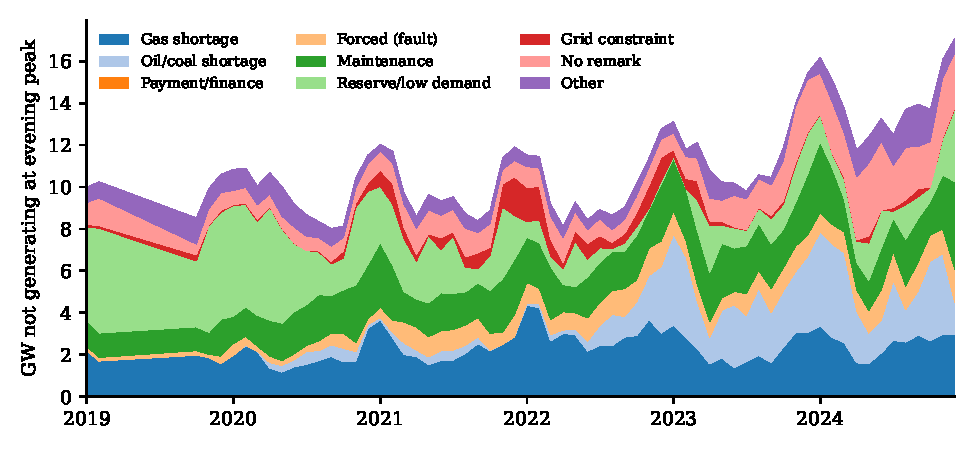
\includegraphics[width=\textwidth]{fig/fig1_lost_capacity.pdf}
\caption{Capacity not generating at the evening peak, by stated cause}\label{fig:lost}
\fignote{Monthly means of daily totals. Off units contribute their capacity; running units contribute capacity minus evening-peak output, attributed to the unit's remark. All grid-connected units, October 2019 -- December 2024.}
\end{figure}

\section{Fleet reliability}

Figure~\ref{fig:lost} decomposes capacity not generating at the evening peak. In 2019--2020 most idle capacity was reserve; from 2022 most was idle for fuel: gas, and from 2023 oil and coal as foreign exchange ran short. Faults and maintenance account for a steady 1--3 GW.

Table~\ref{tab:ieee} reports day-based analogues of IEEE 762 metrics. Because the data are evening-peak snapshots with daily energy, hours are replaced by days and partial outages (derates) by the share of capacity missing at the evening peak on running days whose remark names a fault. EFOR is $(\mathrm{FOD}+\mathrm{EFDD})/(\mathrm{FOD}+\mathrm{SD})$, with forced-outage days FOD, equivalent forced derated days EFDD and service days SD. EAF subtracts forced, maintenance and planned outage days and equivalent derates from active days; a second EAF also subtracts days lost to fuel, finance and grid constraints, which IEEE 762 treats as outside management control (OMC). Combined-cycle units had an EFOR of \ieeeCcEFOR{} and an EAF of \ieeeCcEAF, or \ieeeCcEAFomc{} when fuel shortages are counted; for steam units the fuel-inclusive EAF falls to \ieeeStEAFomc. Single-cycle gas turbines had an EFOR of \ieeeGtEFOR, but \gtTopThreeShare\% of their forced-outage days come from three units out for years (Haripur GT, Shikalbaha peaking GT and Tongi). Derates matter: for combined-cycle units the full-outage forced rate is \ieeeCcFOR{} against an EFOR of \ieeeCcEFOR. Because derates are measured at one evening hour, Table~\ref{tab:sens} reports EFOR without derates, counting only shortfalls of at least 10\% of capacity, and on load-shedding days only, when all available capacity was called and a shortfall cannot be dispatch. Daily snapshots do not map exactly onto hourly GADS definitions, so the metrics are not directly comparable with North American class averages.

\begin{table}[t]
\centering\footnotesize
\caption{Reliability metrics by technology, October 2019 -- December 2024}\label{tab:ieee}
\begin{threeparttable}
% generated from tab_ieee_rows.tex by code/31_numbers.py
\setlength{\tabcolsep}{2.5pt}
\begin{tabular}{lrrrrrrrrrr}
\toprule
 & Units & Active & Inactive & EFOR & EAF & EAF incl. & MTBF & MTTR & Weibull & Crow-AMSAA \\
 & & unit-yrs & (\%) & & & OMC & (svc days) & (median d) & $\beta$ & $\beta$ \\
\midrule
Combined cycle & 37 & 148 & 4 & 0.130 & 0.80 & 0.71 & 290 & 3 & 0.76 & 0.97 \\
Gas turbine & 24 & 102 & 8 & 0.343 & 0.74 & 0.62 & 105 & 1 & 0.69 & 1.18 \\
Steam & 18 & 40 & 27 & 0.075 & 0.81 & 0.58 & 347 & 6 & 0.78 & 0.72 \\
Recip.\ engine$^a$ & 97 & 384 & 0 & 0.081 & 0.93 & 0.88 & 657 & 1 & 0.57 & 1.58 \\
\bottomrule
\end{tabular}



\begin{tablenotes}\footnotesize
\item Day-based analogues of IEEE 762 metrics from evening-peak snapshots. Inactive: spells over 180 days that never name a fault. MTBF: service days per forced outage. MTTR: median forced-outage spell length. Weibull $\beta$: shape of the distribution of service days between failure events (forced-outage onsets and grid-operator-recorded trips), maximum likelihood, pooled across units (per-unit fits in the text). Crow-AMSAA $\beta$: power-law NHPP shape, pooled time-truncated estimator; $\beta>1$ deteriorating, $<1$ improving. $^a$Engine plants are single rows of 10--30 engines; a failed engine shows up as a derate.
\end{tablenotes}
\end{threeparttable}
\end{table}

\begin{table}[t]
\centering\footnotesize
\caption{Sensitivity of reliability metrics to the inactive rule and to the treatment of derates}\label{tab:sens}
\begin{threeparttable}
\begin{tabular}{lccc}
\toprule
 & Combined cycle & Gas turbine & Steam \\
\midrule
\multicolumn{4}{l}{\emph{EAF (inactive share, \%) by inactive threshold}} \\
\quad 90 days & \inactNinetyCcEAF{} (\inactNinetyCcShare) & \inactNinetyGtEAF{} (\inactNinetyGtShare) & \inactNinetyStEAF{} (\inactNinetyStShare) \\
\quad 180 days (main) & \inactOneEightyCcEAF{} (\inactOneEightyCcShare) & \inactOneEightyGtEAF{} (\inactOneEightyGtShare) & \inactOneEightyStEAF{} (\inactOneEightyStShare) \\
\quad 365 days & \inactThreeSixFiveCcEAF{} (\inactThreeSixFiveCcShare) & \inactThreeSixFiveGtEAF{} (\inactThreeSixFiveGtShare) & \inactThreeSixFiveStEAF{} (\inactThreeSixFiveStShare) \\
\quad No inactive class & \inactNoneCcEAF{} (0) & \inactNoneGtEAF{} (0) & \inactNoneStEAF{} (0) \\
\midrule
\multicolumn{4}{l}{\emph{EFOR by treatment of derates}} \\
\quad No derates (FOR) & \eforNoneCc & \eforNoneGt & \eforNoneSt \\
\quad All fault-remark derates (main) & \eforAllCc & \eforAllGt & \eforAllSt \\
\quad Shortfalls $\geq$10\% of capacity only & \eforTenCc & \eforTenGt & \eforTenSt \\
\quad Load-shedding days only & \eforShedCc & \eforShedGt & \eforShedSt \\
\bottomrule
\end{tabular}
\begin{tablenotes}\footnotesize
\item October 2019 -- December 2024. Long spells that name a fault are never classed inactive, so forced-outage rates do not depend on the threshold. Load-shedding days: rate computed on days with load shedding, when all available capacity was called.
\end{tablenotes}
\end{threeparttable}
\end{table}

Pooled across units, times between failure events, measured in service days, follow Weibull distributions with shape parameters below one (combined cycle \wbCc, unit-bootstrap interval \wbBootCcLo--\wbBootCcHi; gas turbine \wbGt; steam \wbSt; engines \wbRe). A pooled shape below one can arise from mixing units with different failure rates even if each unit fails at a constant rate, so I also fit each unit with at least eight intervals separately. The median unit shape is \wbUnitCc{} for combined-cycle units (\wbUnitCcLt\% of \wbUnitCcN{} units below one) and \wbUnitGt{} for gas turbines: failure intervals are close to exponential, with at most mild clustering within units, and most of the pooled shape reflects heterogeneity between units. Repairs are short and skewed: the median forced outage lasts \ieeeCcMTTRmed{} days for combined-cycle units (mean \ieeeCcMTTRmean) and \ieeeStMTTRmed{} for steam units, with long tails from multi-year breakdowns. Power-law (Crow-AMSAA) shapes are \caCc{} for combined-cycle units, \caGt{} for gas turbines, \caRe{} for engine plants and \caSt{} for steam units, and unit-level Laplace tests find deterioration in \lapCcDet{} and improvement in \lapCcImp{} of \lapCcTested{} combined-cycle units. These trend estimates should be read with caution: forced-outage onsets per 1,000 running unit-days rose from \onsetRateNineteen{} in 2019 to \onsetRateTwentyFour{} in 2024 while trips fell from \tripRateNineteen{} to \tripRateTwentyFour, a divergence that may reflect changes in how outages were labelled rather than in equipment.

\section{Methods}

Comparisons between units use, for unit $i$ of technology $k$ on day $t$,
\begin{equation}
y_{it} = \beta\,\mathrm{Private}_i + \sum_a \gamma_a \mathbf{1}[\mathrm{age}_{it}\in a] + \theta \log \mathrm{cap}_i + \delta_{k,m(t)} + \varepsilon_{it},
\end{equation}
with technology-by-year-month fixed effects $\delta_{k,m(t)}$, so that units are compared with others of the same technology in the same month, under the same fuel-supply conditions. Outcomes are the forced state (per 1,000 days, among days running or in forced outage), trips (per 1,000 unit-days that ran the day before), non-fuel unavailability (\% of active days off for a reason other than fuel, finance, reserve or contract) and two measures that ignore the remarks: the share of days with zero output, and the same share excluding only reserve, contract and inactive days. Standard errors are clustered by unit; because only about a dozen units are private, $p$-values from a wild cluster restricted bootstrap with Webb weights (4,999 draws, each bootstrap outcome re-partialled on the fixed effects and controls) are also reported.

Weather effects are estimated within units with Poisson regressions of daily counts of trips and forced-outage onsets, among units that ran the day before:
\begin{equation}
\log \mathbb{E}[y_{it}] = \sum_{b} \beta_b \mathbf{1}[T^{\max}_{it}\in b] + \lambda P_{it} + \gamma' X_{it} + \alpha_i + \delta_{m(t)},
\end{equation}
with temperature bins $b$ (reference 30--33\,\textdegree C) or linear temperature, precipitation $P_{it}$ (per 10 mm), humidity, system demand relative to its monthly mean and a load-shedding indicator, unit fixed effects $\alpha_i$ and year-month fixed effects. Bin coefficients are reported with Holm-adjusted $p$-values. Repair durations are analysed with a Cox model of the hazard of returning to service.

\section{Results}

\subsection{Private and state-owned units}

\begin{table}[t]
\centering\small
\caption{Private versus state-owned large thermal units}\label{tab:own}
\begin{threeparttable}
\setlength{\tabcolsep}{4pt}
\begin{tabular}{lrrrrrr}
\toprule
Outcome & Mean & Private & (s.e.) & $p$ (CRV) & $p$ (wild) & Units (private) \\
\midrule
Forced state, per 1,000 days & \ownForcedMean & \ownForcedB & (\ownForcedSE) & \ownForcedP & \ownForcedPw & \ownForcedUnits{} (\ownForcedPrivUnits) \\
Trips, per 1,000 unit-days & \ownTripMean & \ownTripB & (\ownTripSE) & \ownTripP & \ownTripPw & \ownTripUnits{} (\ownTripPrivUnits) \\
Non-fuel unavailability, \% & \ownNonfuelMean & \ownNonfuelB & (\ownNonfuelSE) & \ownNonfuelP & \ownNonfuelPw & \ownNonfuelUnits{} (\ownNonfuelPrivUnits) \\
Zero output, any reason, \% & \ownZeroMean & \ownZeroB & (\ownZeroSE) & \ownZeroP & \ownZeroPw & \ownZeroUnits{} (\ownZeroPrivUnits) \\
Zero output excl.\ reserve etc., \% & \ownZeroExclMean & \ownZeroExclB & (\ownZeroExclSE) & \ownZeroExclP & \ownZeroExclPw & \ownZeroExclUnits{} (\ownZeroExclPrivUnits) \\
\midrule
Forced state, combined cycle only & \ownCcgtMean & \ownCcgtB & (\ownCcgtSE) & \ownCcgtP & \ownCcgtPw & \ownCcgtUnits{} (\ownCcgtPrivUnits) \\
Trips, combined cycle only & \ownCcgtTripMean & \ownCcgtTripB & (\ownCcgtTripSE) & \ownCcgtTripP & \ownCcgtTripPw & \ownCcgtTripUnits{} (\ownCcgtTripPrivUnits) \\
Forced state, excluding steam & \ownNoSteamMean & \ownNoSteamB & (\ownNoSteamSE) & \ownNoSteamP & \ownNoSteamPw & \ownNoSteamUnits{} (\ownNoSteamPrivUnits) \\
Idle for fuel or finance, \% & \ownFuelIdleMean & \ownFuelIdleB & (\ownFuelIdleSE) & \ownFuelIdleP & -- & \ownFuelIdleUnits{} (\ownFuelIdlePrivUnits) \\
\bottomrule
\end{tabular}
\begin{tablenotes}\footnotesize
\item Linear probability models with technology $\times$ year-month fixed effects (year-month only for single-technology rows), controlling for age bins and log capacity (zero-output and fuel rows include undated units and control for log capacity only). Combined-cycle, single-cycle gas turbine and steam units, October 2019 -- December 2024. ``Excl.\ reserve etc.'': excluding reserve, contract-expiry and inactive days. CRV: standard errors clustered by unit. Wild: wild cluster restricted bootstrap, Webb weights, 9,999 draws. There are no private single-cycle gas turbines.
\end{tablenotes}
\end{threeparttable}
\end{table}

Table~\ref{tab:own} compares private and state-owned units of the same technology in the same month. The private--public difference in forced-outage days is \ownForcedB{} per 1,000 days, on a mean of \ownForcedMean{} (wild-bootstrap $p=\ownForcedPw$); dropping one private unit at a time keeps it between \ownLooLo{} and \ownLooHi, and it is similar without steam units (\ownNoSteamB). Among combined-cycle units alone it is \ownCcgtB{} on a mean of \ownCcgtMean{} but imprecise (wild $p=\ownCcgtPw$). Part of the gap comes from multi-year breakdowns of a few public units, which a private owner might have repaired or retired. Private units also had fewer trips recorded by the grid operator and less non-fuel unavailability, but neither difference is statistically significant (trips \ownTripB{} per 1,000 unit-days, mean \ownTripMean, wild $p=\ownTripPw$; non-fuel unavailability \ownNonfuelB{} points, mean \ownNonfuelMean, wild $p=\ownNonfuelPw$). Private units were not idled for fuel significantly less often (difference \ownFuelIdleB{} points, $p=\ownFuelIdleP$), so the gap does not reflect priority in gas allocation. The metrics agree: among combined-cycle units EFOR was \ieeeCcPrivEFOR{} for private and \ieeeCcPubEFOR{} for public units, and mean service days between forced outages \ieeeCcPrivMTBF{} against \ieeeCcPubMTBF. After an outage, the hazard of returning to service was \coxPrivHR{} times that of public units ($p=\coxPrivP$; \coxPrivN{} private spells).

Private producers are paid for declared availability and could describe outages favourably. The incentive matters most for a fault labelled as fuel shortage, which under Bangladeshi power purchase agreements shifts the risk to the buyer. The zero-output measure that ignores all labels gives a private--public difference of \ownZeroB{} points in the share of zero-output days (mean \ownZeroMean; wild $p=\ownZeroPw$); excluding reserve, contract and inactive days the difference is \ownZeroExclB{} points ($p=\ownZeroExclP$). Trips, which the grid operator records, point the same way. The label-free and operator-recorded measures are thus consistent in sign with the forced-state gap but too imprecise to confirm it.

The comparison does not identify an effect of ownership. Private and public units differ in vintage, manufacturer and design; the identifying variation comes from \nPrivCcgt{} private combined-cycle units, of which two date from 2001--2002 and the rest from 2015 onwards, and two recent private coal-fired steam units. The evidence is that private units in this fleet spent fewer days in forced outage, mostly because they avoided the very long breakdowns seen at some public units; it is suggestive rather than conclusive.

\subsection{Weather and system conditions}

\begin{figure}[t]
\centering
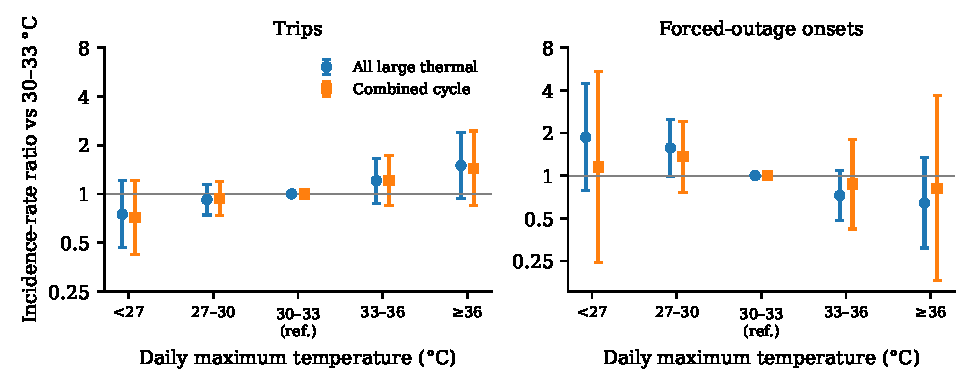
\includegraphics[width=\textwidth]{fig/fig3_heat.pdf}
\caption{Trips and forced-outage onsets by daily maximum temperature}\label{fig:heat}
\fignote{Incidence-rate ratios from Poisson regressions with unit and year-month fixed effects and controls for humidity, precipitation, demand deviation and load shedding; 95\% confidence intervals, standard errors clustered by unit. Reference 30--33\,\textdegree C. Large thermal units that ran the day before.}
\end{figure}

Within a unit and month, daily maximum temperature varies with a standard deviation of only \tmaxSDwithin\,\textdegree C (\tmaxSDraw\,\textdegree C overall), and the sample contains \heatTrips{} trips and \heatOnsets{} forced-outage onsets in \heatUnitDays{} unit-days, so power is limited. Trips rise with temperature but not significantly: the incidence-rate ratio is \heatTripIRR{} per \textdegree C (95\% CI \heatTripIRRLo--\heatTripIRRHi) and \hotTripIRR{} above 36\,\textdegree C (\hotTripIRRLo--\hotTripIRRHi; \heatTripsHot{} trips). Forced-outage onsets \emph{fall} with temperature (\heatOnsetIRR{} per \textdegree C, \heatOnsetIRRLo--\heatOnsetIRRHi, $p=\heatOnsetIRRP$), although no individual bin is significant after Holm adjustment (Figure~\ref{fig:heat}). The decline is more plausibly operational than physical: on hot days demand peaks, units are kept running through minor problems and discretionary repairs are deferred, much as days of high system demand are associated with fewer trips (\demB{} per 1,000 per GW above the monthly mean, s.e.\ \demSE). These estimates do not support a material effect of heat on forced outages in this climate, but cannot rule out a moderate increase in trips at the hottest temperatures.

\begin{figure}[t]
\centering
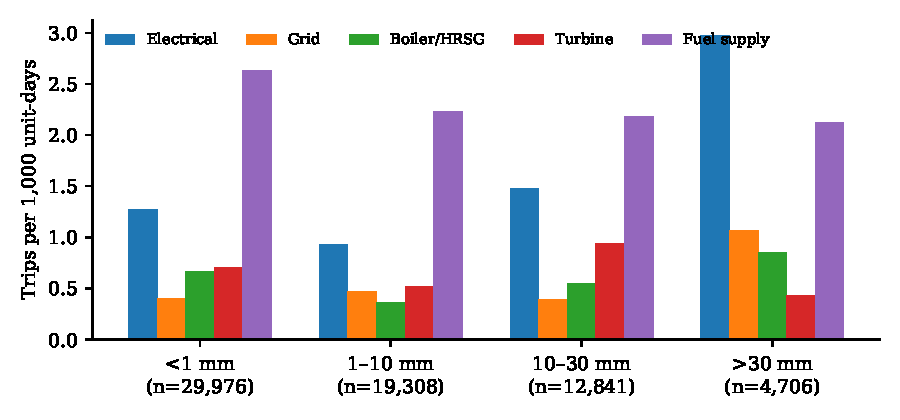
\includegraphics[width=0.92\textwidth]{fig/fig2_rain_causes.pdf}
\caption{Generator trips by stated cause and daily precipitation}\label{fig:rain}
\fignote{Large thermal units that ran the day before, October 2019 -- December 2024. Trips with unstated or other causes are not shown. Precipitation from NASA POWER at the unit's location.}
\end{figure}

Rain raises trips: each 10 mm multiplies the trip rate by \rainTripIRR{} (95\% CI \rainTripIRRLo--\rainTripIRRHi, $p\rainTripIRRP$), about \rainLpmB{} trips per 1,000 unit-days per mm on a mean of \tripMean, and the effect holds for combined-cycle units alone (\rainTripCcgtIRR). It does not raise forced-outage onsets (\rainOnsetIRR). Cause-specific Poisson models locate the effect (Figure~\ref{fig:rain}): electrical trips rise by a factor of \rainElec{} per 10 mm (\rainElecLo--\rainElecHi, $p\rainElecP$, \rainElecN{} events), while mechanical trips (turbine, boiler and cooling; \rainMech, \rainMechN{} events), control (\rainCtrl) and grid trips (\rainGrid, \rainGridN{} events) show no detectable change and fuel-supply trips a marginal rise (\rainFuel, 95\% CI \rainFuelLo--\rainFuelHi). The pattern is consistent with lightning, moisture in electrical equipment and switching disturbances; lightning-flash data would allow a sharper test.

\subsection{Age and repair}
Units aged 20 years or more spent \ageOldB{} more days per 1,000 in forced outage than units aged 5--9 (s.e.\ \ageOldSE, $p=\ageOldP$), but this rests on few old units, and earlier corrections of two commissioning dates changed raw age patterns substantially. Excluding commissioning test days, new units show no excess non-fuel unavailability (\newUnitB{} points, $p=\newUnitP$). In the Cox model of repair, old units return to service more slowly (hazard ratio \coxOldHR, $p=\coxOldP$), as do steam units (\coxSteamHR) and spells recorded only as unspecified maintenance (\coxUnspecHR), while single-cycle gas turbines return faster (\coxGTHR).

\section{Discussion}

Public dispatch reports support reliability statistics at the level of the generating unit, provided the parsed figures are checked against printed totals and the stated causes against independent series. For Bangladesh in 2019--2024 they show a fleet whose availability was limited more by fuel than by equipment: the fuel-inclusive availability of combined-cycle units was nine points below their equipment availability, and for steam units more than twenty. Equipment failures occur at close to constant rates within units, with large differences between units, short typical repairs and long tails of multi-year breakdowns.

Private units spent fewer days in forced outage, but the gap is driven partly by long public breakdowns, is imprecise in several checks and compares two fleets of different vintage and design. The rain result has a specific mechanism, electrical faults, relevant to protection and lightning design at plants and substations. The absence of a heat effect on forced outages contrasts with the temperature dependence found in the United States \citep{murphy2019timedependent}; it may reflect the narrow temperature range of a humid tropical climate, the coarse temperature measure, the dominance of fuel constraints under which heat-sensitive units are often idle, and the deferral of repairs on peak days.

Several limitations apply. The reports are evening-peak snapshots with daily energy, so short outages appear only as trips and derates are measured at one hour. Remarks are written by plants and dispatchers and are not audited, and maintenance is rarely labelled planned. Trip links and remark codes have been checked by the author on samples but not yet by an independent coder. Commissioning years are uncertain for the oldest units. The reporting change of January 2025 limits the main sample to five years and three months; repeating the analysis on 2025--26 once remarks are reconstructed would test the results out of sample.

\section{Conclusion}

Public daily reports from Bangladesh's grid operator yield a validated unit-level record of availability, outage causes and generator trips for a national fleet. Over 2019--2024, fuel, not equipment, was the main reason thermal capacity stood idle; combined-cycle units had an EFOR of about \ieeeCcEFOR{} with failure rates that differ widely between units; private units tended to spend fewer days in forced outage than state-owned units of the same technology; rain raised electrical trips; and daily heat did not increase forced outages. The approach can be applied wherever dispatch reports are published.

\bibliographystyle{plainnat}
\bibliography{refs}

\end{document}
